\section{Software Development Process}
\label{sec:SoftwareDevelopmentProcess}

\subsection{Overview} 
The process of developing software is an extensive and complex process that requires a lot of planning, both in relation to the methodologies used during the development process and the requirements, both functional and non-functional of the software. This section details life cycle models considered for NeuraViz's development, the model that was eventually chosen, and modifications to the model necessary for the development of this particular system. It also lays out functional and non-functional requirements for NeuraViz.

\subsection{Life Cycle Model}
Prior to beginning development of NeuraViz, a number of software life cycle models were considered to govern the pace and structure of development. In all the waterfall model, iterative model, and agile model were considered. More specifically with agile, a variation of scrum, modified for a single developer, was considered. Ultimately, the modified scrum model was chosen for its flexibility and ability to adapt quickly to changing requirements.

\subsubsection{Waterfall Model}
% TODO: Add citation (Gagan2020)
The waterfall model is one of the oldest software development lifecycle (SDLC) models, originally proposed by Winston Royce in 1970. The model is a linear, sequential approach to software development, with each phase of the development process directly following the previous phase. Each subsequent phase relies on the previous phase, and as such the model does not allow going back to previous phases once they are completed. The first phase of the waterfall model is the requirement analysis phase, in which project requirements, both functional and non-functional, are gathered and documented. At this phase, requirements are also often analyzed for traits like consistency and feasibility. The second phase is the system design phase, in which the architecture of the software system is designed in full. All details of what needs to be done and how it will be completed are considered and documented during this phase. Third, the implementation phase is where the code for the software is written and the design from the previous step is implemented in full, exactly as specified during the design phase. During the fourth phase, the software is tested for bugs and errors, and issues are resolved as needed. Fifth, the software is deployed to the client in its entirety. In the waterfall model, this is the first time the client has seen the software. Finally, the software is maintained and updated as needed for as long as the client needs it.

Because of its rigid structure, the waterfall model excels at being very easy to understand and pick up quickly for new developers. In addition, it is easy to manage with relatively little overhead in management. When project requirements are well understood up front and unlikely to change, the waterfall model also serves the benefit of ensuring design is completed before implementation begins, which leads to fewer mistakes and less necessity to change the code once it has been written. However, for projects where requirements are less well understood or are likely to change, the waterfall model struggles to adapt and may lead to a design that was flawed in the first place with no way to fix it. In addition, the waterfall model does not allow for client feedback until the software is fully completed, which can lead to a lot of wasted time and effort if the client is not satisfied with the final product. 

% TODO: Add citation (tutorialspointWaterfall)
\begin{figure}[htb]
    \centering
    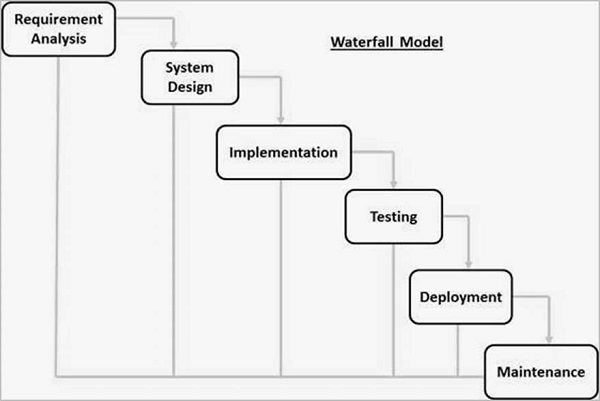
\includegraphics[width=.75\textwidth]{02_dev_process/res/sdlc_waterfall_model.jpg}
    \caption[Waterfall Model Diagram]{Waterfall Model Diagram}
\end{figure}

\subsubsection{Iterative Model}
% TODO: Add iterative model
Like the waterfall model, the iterative model is mostly linear and sequential with a relatively rigid structure where each step directly follows the previous step. The phases in the iterative model roughly match those in the waterfall model, including a requirements analysis phase, a design phase, and implementation phase, a testing phase, and a deployment phase. Unlike the waterfall model, however, the iterative model runs these phases, with the exception of requirements analysis, multiple times, restarting the sequence of phases after each deployment. This serves the major benefit of allowing the ability for the client to give feedback on the project sooner and more often.

Due to its similarity to the waterfall model, the iterative model exhibits many of the same benefits of waterfall in that it is easy to understand with a relatively linear structure and minimal overhead. Like the waterfall model, when requirements are understood at the project outset, the design is likely to be almost fully complete before development begins, so the code is also less likely to require changes later in the process. While the iterative model does improve on the waterfall model's lack of ability for client feedback, it still struggles with changing requirements as each iteration of the project is still long and expected to be a relatively complete implementation of the software.

% TODO: Add citation (tutorialspointIterative)
\begin{figure}[htb]
    \centering
    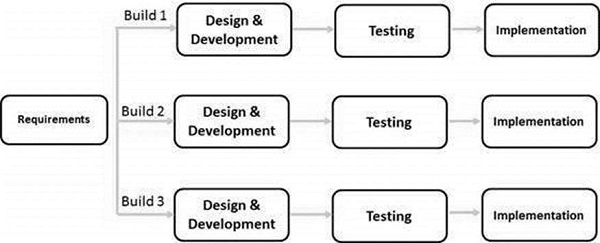
\includegraphics[width=0.75\textwidth]{02_dev_process/res/sdlc_iterative_model.jpg}
    \caption[Iterative Model Diagram]{Iterative Model Diagram}
\end{figure}

\subsubsection{Agile (Scrum) Model}
% TODO: Add Agile model

\subsection{Requirements}
% TODO: Add Requirements
